\documentclass[border=10pt]{standalone}

\usepackage{tikz}
\usepackage{tikzsymbols}
\usetikzlibrary{calc,patterns,shapes.geometric}

\def\centerarc[#1](#2)(#3:#4:#5){\draw[#1] ($(#2)+({#5*cos(#3)},{#5*sin(#3)})$) arc (#3:#4:#5);}

\begin{document}
	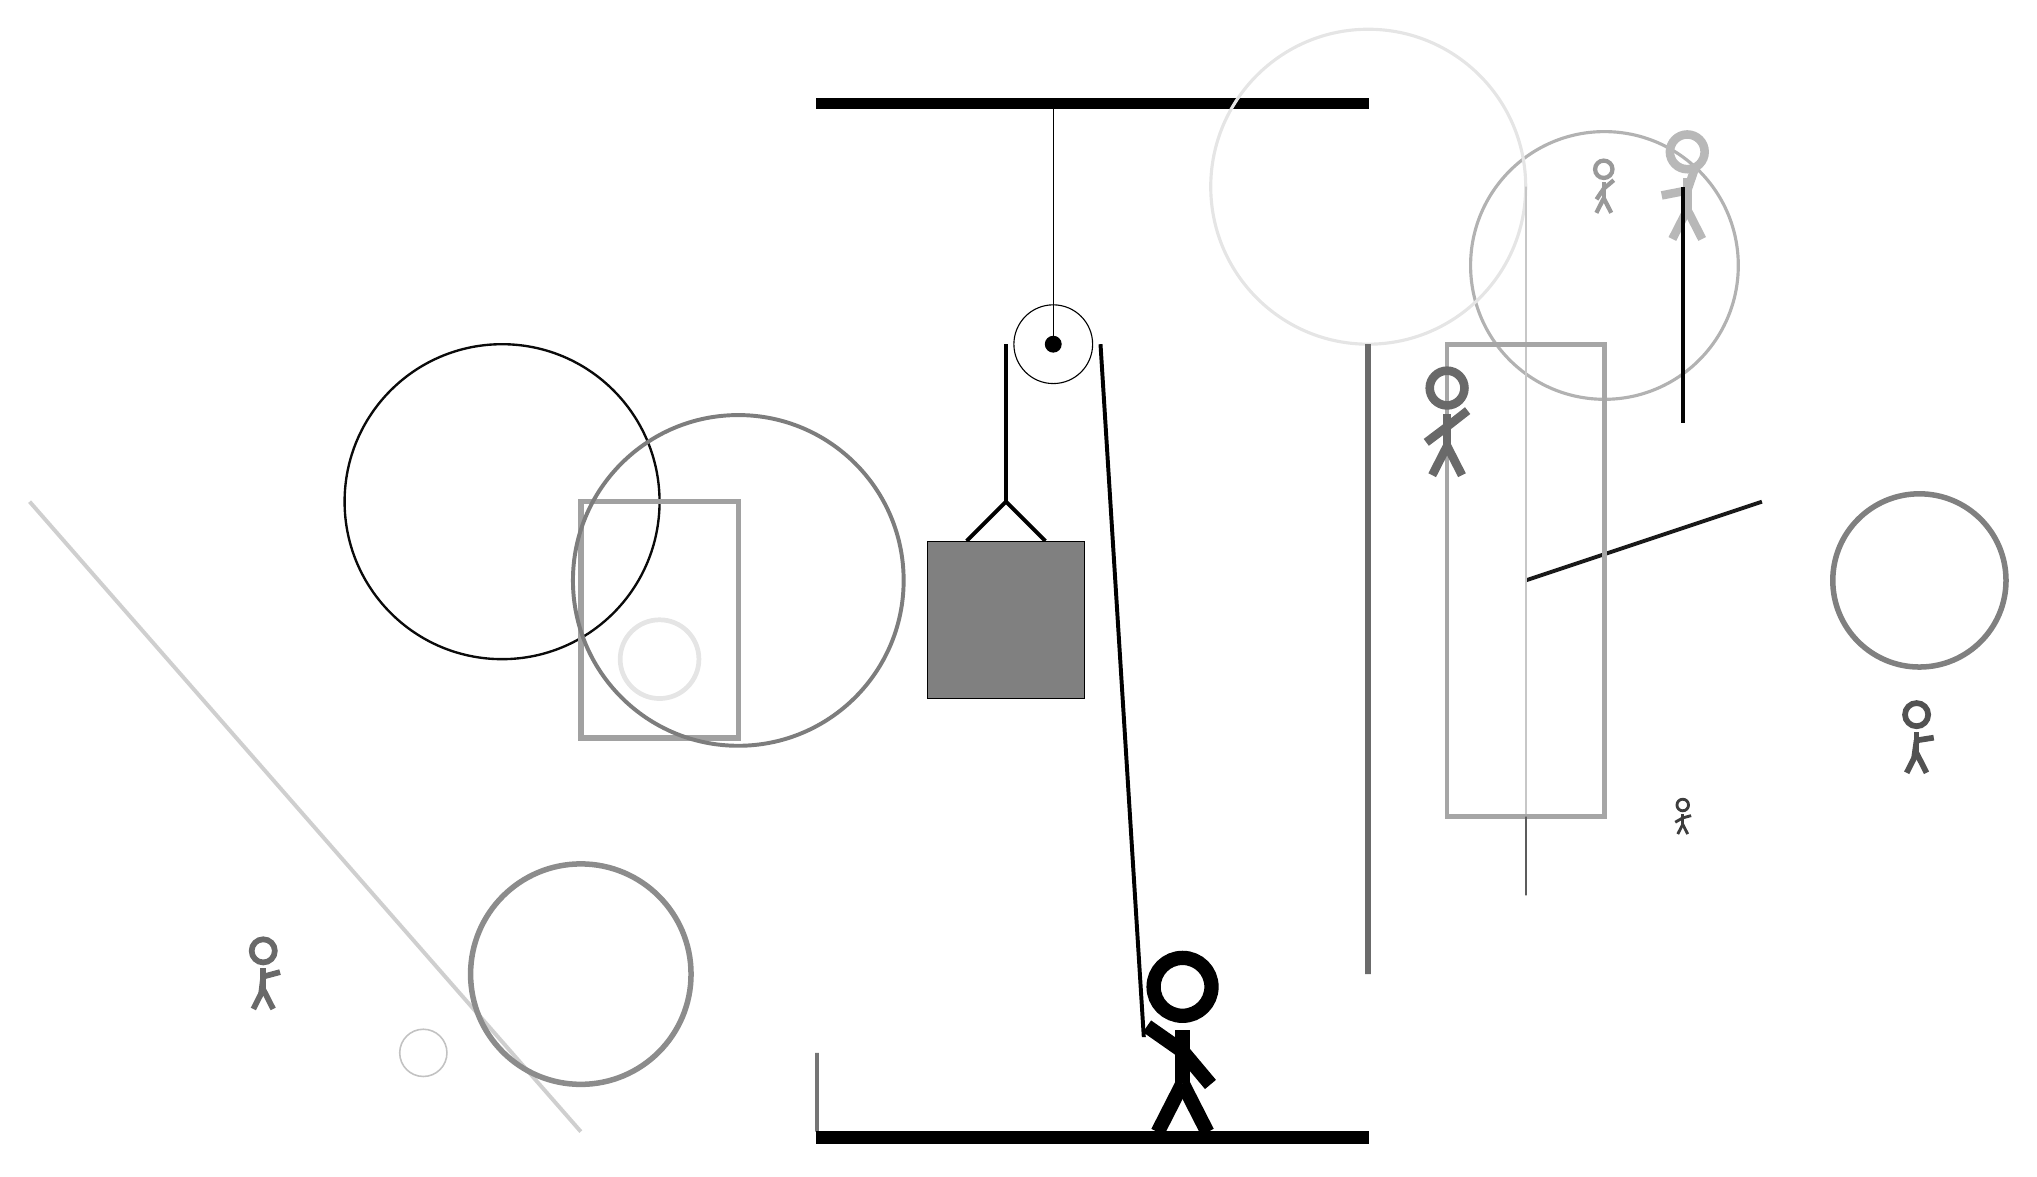
\begin{tikzpicture}
		%%%%% START %%%%%
		
		\draw[fill=black] (-2, 10) rectangle (5, 10.125);
		
		\draw [line width=0.3mm, color=black!96](-6, 5) circle (2.0);
		
		\draw [line width=0.3mm, color=black!48](9, 5) circle (0.0);
		\draw[line width=0.7mm, color=black!37] (-3, 2) rectangle (-5, 5);
		\draw[line width=0.6mm, color=black!54] (-2, -2) rectangle (-2, -3);
		
		\draw[line width=0.5mm, color=black!90](7, 4) -- (10, 5);
		\draw [line width=0.4mm, color=black!30](8, 8) circle (1.7);
		\draw [line width=0.4mm, color=black!10](5, 9) circle (2.0);
		
		\draw[line width=0.7mm, color=black!58] (5, 7) rectangle (5, -1);
		\draw [line width=0.3mm, color=black!17](11, 6) circle (0.0);
		\node[line width=0.7mm, color=black!28] at (9, 9) {\Strichmaxerl[6][11][71]};
		\draw [line width=0.6mm, color=black!10](-4, 3) circle (0.5);
		\draw[line width=0.5mm, color=black!19](-5, -3) -- (-12, 5);
		\draw[line width=0.3mm, color=black!22] (7, 1) rectangle (7, 9);
		
		\draw [line width=0.5mm, color=black!51](-3, 4) circle (2.1);
		\node[line width=0.6mm, color=black!59] at (-9, -1) {\Strichmaxerl[4][83][15]};
		\node[line width=0.3mm, color=black!68] at (12, 2) {\Strichmaxerl[4][82][9]};
		
		\draw[line width=0.5mm, color=black!98](9, 6) -- (9, 9);
		\draw [line width=0.7mm, color=black!45](-5, -1) circle (1.4);
		\node[line width=0.2mm, color=black!76] at (9, 1) {\Strichmaxerl[2][30][15]};
		
		\draw[line width=0.6mm, color=black!35] (6, 7) rectangle (8, 1);
		\node[line width=0.2mm, color=black!59] at (6, 6) {\Strichmaxerl[6][37][38]};
		
		\node[line width=0.7mm, color=black!40] at (8, 9) {\Strichmaxerl[3][56][40]};
		\draw [line width=0.2mm, color=black!24](-7, -2) circle (0.3);
		\draw [line width=0.7mm, color=black!50](12, 4) circle (1.1);
		\draw[line width=0.3mm, color=black!64] (7, 0) rectangle (7, 1);
		
		\draw (1, 7) circle (0.5);
		\draw[fill=black] (1, 7) circle (0.1);
		\draw (1, 10) -- (1, 7);
		
		\draw[line width=0.5mm] (-0.1, 4.5) -- (0.4, 5.0) -- (0.9, 4.5);
		\draw[fill=black!50] (-0.6, 4.5) rectangle (1.4, 2.5);
		
		\draw[line width=0.5mm] (0.4, 7) -- (0.4, 5.0);
		\centerarc[line width=0.5mm](1, 7)(0:180:0.6);
		\draw[line width=0.5mm](1.6, 7) -- (2.15, -1.8);
		
		\node at (2.6, -1.9) {\Strichmaxerl[10][-35][-50]};
		
		\draw[fill=black] (-2, -3) rectangle (5, -3.15);
		
		%%%%% END %%%%%
	\end{tikzpicture}
\end{document}